
\begin{figure}[t]
    \centering
    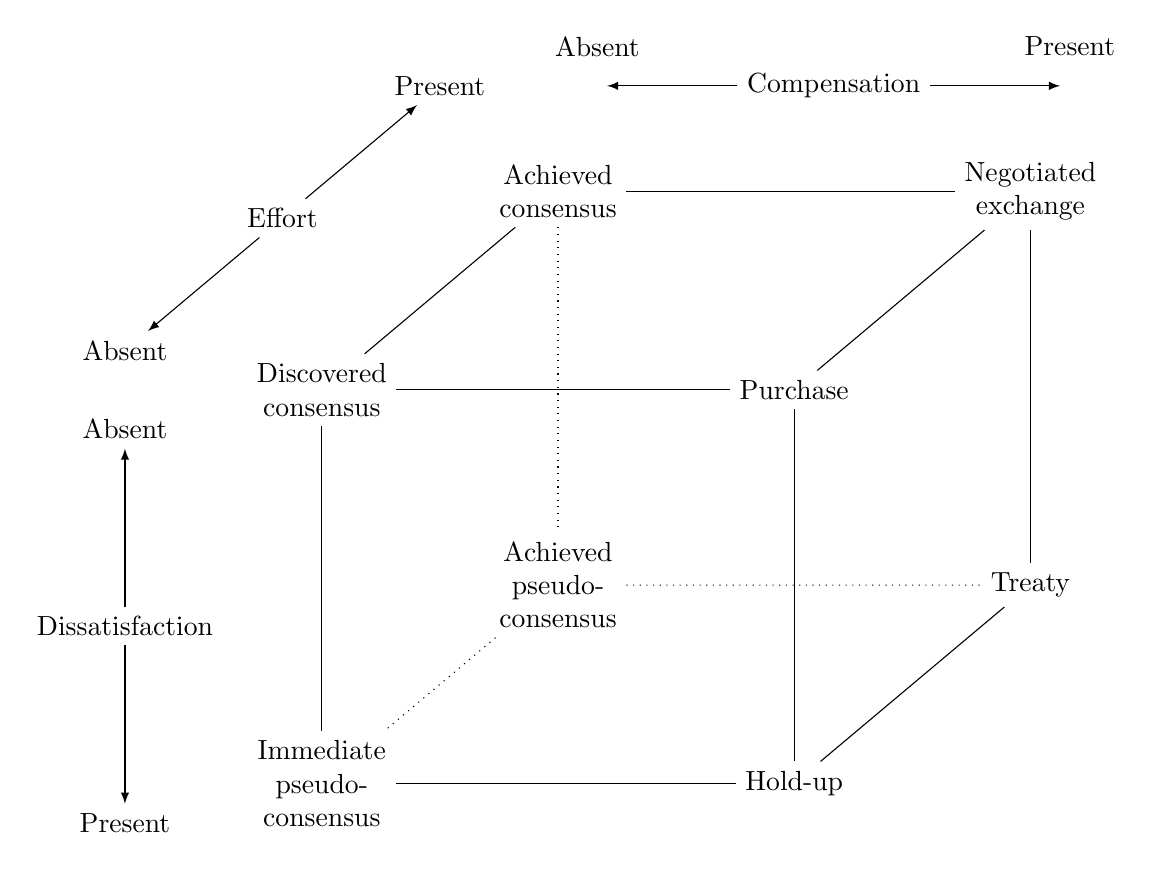
\begin{tikzpicture}
        % Put Effort (Absent) at origin plus a little movement back.
        % Cube corner is at origin
        % 40 degrees e.g. tan(40 degrees) * x = y
        \draw (-2.5,0.5) ++(2cm,1.68cm) node (Effort) {Effort};
        \draw (Effort) ++(-2cm,-1.68cm) node (EffortAbsent) {Absent}
              (Effort) ++(2cm,1.68cm) node (EffortPresent) {Present};

        \draw (EffortPresent) ++(5cm,0) node (Compensation) {Compensation}
              (Compensation) ++(-3,0) node (CompensationAbsent) {}
              ++(0,0.5) node {Absent}
              (Compensation) ++(3,0) node (CompensationPresent) {}
              ++(0,0.5) node {Present};


        \draw (-2.5,-0.5) ++(0,-2.5cm) node (Dissatisfaction) {Dissatisfaction}
            (Dissatisfaction) ++(0,2.5cm) node (DissatisfactionAbsent) {Absent}
            (Dissatisfaction) ++(0,-2.5) node (DissatisfactionPresent) {Present};

        \foreach \x in {Compensation,Effort,Dissatisfaction}
        \foreach \y in {Absent,Present}
        {
            \draw [->,>=latex] (\x) -- (\x\y);
        }

        \node (Cube) at (0,0) {};

        \draw (Cube) node [align=center] (DiscoveredConsensus) {Discovered \\ consensus}
            ++(3cm,2.52cm) node [align=center] (AchievedConsensus) {Achieved \\ consensus}
            ++(6cm,0) node [align=center] (NegotiatedExchange) {Negotiated \\ exchange}
            (DiscoveredConsensus) ++(6cm,0) node[align=center] (Purchase) {Purchase}
            (DiscoveredConsensus) ++(0,-5cm) node[align=center] (ImmediatePC) {Immediate \\ pseudo-\\consensus}
            (Purchase) ++(0,-5cm) node[align=center] (HoldUp) {Hold-up}
            (NegotiatedExchange) ++(0,-5cm) node[align=center] (Treaty) {Treaty}
            (AchievedConsensus) ++(0,-5) node[align=center] (AchievedPC) {Achieved\\pseudo-\\consensus};

        \foreach \x[remember=\x as \lastx (initially Purchase)] in {DiscoveredConsensus,AchievedConsensus,NegotiatedExchange,Purchase,HoldUp,Treaty,NegotiatedExchange}
        {
            \draw (\lastx) -- (\x);
        }
        \foreach \x[remember=\x as \lastx (initially DiscoveredConsensus)] in {ImmediatePC,HoldUp}
        {
            \draw (\lastx) -- (\x);
        }
        \foreach \x[remember=\x as \lastx (initially AchievedConsensus)] in {AchievedPC,Treaty}
        {
            \draw [dotted] (\lastx) -- (\x);
        }
        \foreach \x[remember=\x as \lastx (initially AchievedPC)] in {ImmediatePC}
        {
            \draw [dotted] (\lastx) -- (\x);
        }
    \end{tikzpicture}
    \caption{\label{fig:ao-outcome-submodes}Locations of sub-modes in the agreement-on-outcome family \autocite[15]{Tideman2006}.}
\end{figure}